\section{Contexte et cadre de l'étude}
\label{sec:context}

La séparation d’étages constitue un événement critique du vol d’un lanceur multi-étages, dont la réussite conditionne directement
la poursuite nominale de la mission. Dans le cas des lanceurs expérimentaux et des fusées sondes, cette problématique s’inscrit
dans un contexte spécifique, marqué par des contraintes fortes de simplicité, de fiabilité, de coût et de cadre réglementaire,
qui distinguent ces systèmes des lanceurs orbitaux industriels.\\

Cette première partie vise à établir le cadre technique et conceptuel nécessaire à l’étude menée dans le cadre du PMI. Elle
présente tout d’abord les enjeux généraux liés à la séparation d’étages, puis propose une synthèse des principaux principes et
solutions existantes, afin de situer l’approche explorée au regard de l’état de l’art. Les limites rencontrées par ces solutions
dans le contexte des lanceurs expérimentaux sont ensuite discutées, permettant de justifier l’intérêt d’une étude dédiée à une
séparation assistée par l’aérofreinage.\\

Enfin, cette partie introduit le lanceur SP-02 en tant que système hôte de l’étude. Cette présentation est volontairement
synthétique et se limite aux éléments géométriques, structurels et aérodynamiques nécessaires à la compréhension des hypothèses
de modélisation retenues. Elle ne constitue pas une description exhaustive du projet SP-02, mais définit le cadre réaliste dans
lequel s’insèrent les analyses développées dans les sections suivantes.

\subsection{Problématique de la séparation d’étages dans les lanceurs expérimentaux}
\label{sec:problematique}

Un lanceur multi-étages est un véhicule spatial constitué de plusieurs segments successifs (étages) qui se détachent les uns
après les autres au cours du vol pour optimiser la masse propulsée et améliorer les performances. La séparation d’étages est la
transition mécanique et dynamique entre deux étages consécutifs, qui doit être réalisée de manière fiable et contrôlée pour
assurer la continuité de la mission en cours. Cette étape critique du vol implique des défis techniques majeurs, notamment en
termes de génération des forces nécessaires au détachement, de gestion des interactions aérodynamiques et de maintien de la
stabilité du véhicule.

\begin{quote}
    \textit{\og{}A separation mechanism that does not meet these requirements can produce attitude errors and tumble rates of the
    continuing body that are too large for its attitude-control system to accommodate, can damage its structure and critical
    equipment, and can cause failure or degradation of the mission.\fg{}}
    (cf. NASA Flight Separation Mechanisms\cite{NASA_Flight_Separation}).\\
\end{quote}

\begin{figure}[h!]
    \centering
    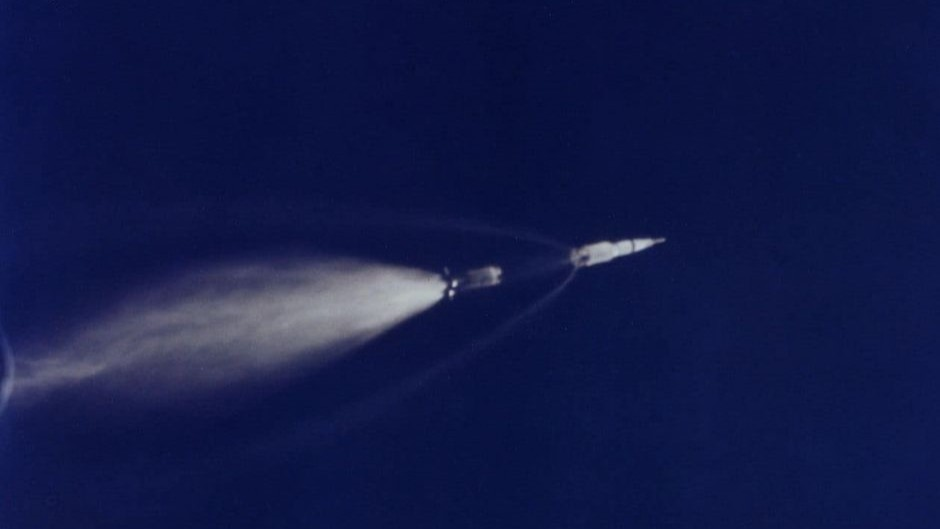
\includegraphics[width=0.9\textwidth]{figures/How-did-the-Saturn-V-stages-separate.jpg}
    \caption{Séparation des étages 1 et 2 du lanceur Saturn V~\cite{SaturnV_Separation}}
\end{figure}

Dans le domaine spatial industriel et commercial, les lanceurs (tels qu’Ariane 6, Falcon 9 ou Electron) exploitent des solutions
de séparation robustes et standardisées, souvent pyrotechniques, intégrées à des processus de qualification lourds. Ces systèmes
sont conçus pour une répétabilité élevée, des milliers d’heures de certification et des procédures de sûreté strictes. La taille,
la complexité et les ressources disponibles (budget, moyens d’essais, expertise) diffèrent radicalement de ceux des projets non
industriels.\\

À l’opposé se trouvent les lanceurs expérimentaux et les fusées sondes :
\begin{itemize}
    \item Un lanceur expérimental désigne généralement un véhicule développé dans un cadre académique ou associatif pour tester
    des concepts technologiques ou atteindre une performance définie dans des gammes de faible coût et faible volume.
    \item Une fusée sonde fait référence à un type de lanceur suborbital utilisé pour des missions scientifiques, des essais en
    atmosphère ou des validations de capteurs, souvent dans le contexte de programmes étudiants, de clubs aérospatiaux ou de
    projets de recherche gouvernementaux à budget limité.\\
\end{itemize}

Ces catégories se caractérisent par des échelles de taille et de masse très différentes des lanceurs commerciaux. Par exemple,
une fusée sonde ou expérimentale peut mesurer quelques mètres pour quelques dizaines de kilogrammes, alors qu’un lanceur orbital
pèse plusieurs centaines de tonnes et dépasse des dizaines de mètres de hauteur. Cette différence d’échelle se reflète directement
dans :
\begin{itemize}
    \item la simplicité de conception,
    \item les moyens de test disponibles,
    \item les contraintes réglementaires applicables,
    \item les budgets alloués,
    \item et les exigences de fiabilité opérationnelle.\\
\end{itemize}

\begin{figure}[h!]
    \centering
    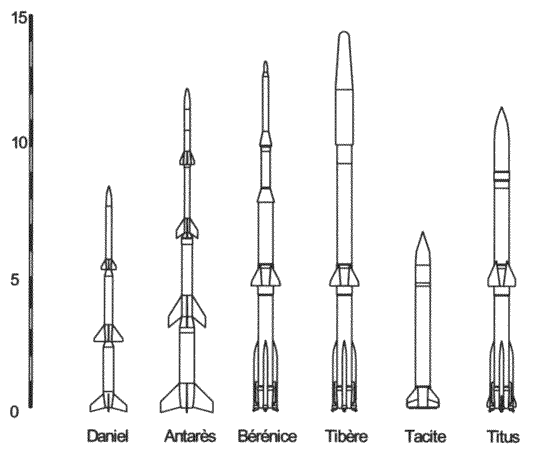
\includegraphics[width=0.6\textwidth]{figures/onera.png}
    \caption{Famille de lanceurs expérimentaux et de fusées sondes développés par l'ONERA~\cite{Onera_Family}}
\end{figure}

Dans ce contexte, la séparation d’étages représente un défi particulier. Les solutions héritées du domaine industriel
(pyrotechnique ou très mécanisées) ne sont pas toujours adaptées à des véhicules de petite échelle, car elles peuvent être
surdimensionnées en termes de charge ou de complexité, nécessiter des procédures d’essai lourdes difficiles à exécuter avec des
moyens limités ou imposer des coûts prohibitif pour des projets à budget restreint.\\

La problématique étudiée dans ce rapport vise donc à comprendre et analyser les solutions possibles de séparation adaptées à ces
contraintes particulières : simplicité, intégration minimale, facilité de test, et compatibilité avec des processus de
développement itératifs. Cette réflexion justifie une investigation des principes existants, suivie d’une exploration dédiée de
solutions compatibles avec les objectifs et la philosophie des lanceurs expérimentaux et des fusées sondes.

\subsection{Principes et état de l’art des systèmes de séparation d’étages}
\label{sec:etat_art_separation}

La littérature technique et scientifique distingue les dispositifs de séparation d’étages selon deux grands critères : le mode
d’activation et la nature des efforts mobilisés pour obtenir une séparation fiable entre les segments du lanceur.

\subsubsection{Modes de séparation d’étages}

\subsubsubsection{Pyrotechnique}

Les dispositifs pyrotechniques représentent une des méthodes les plus répandues dans l’industrie spatiale pour séparer des
étages. Ils reposent sur l’utilisation de charges explosives intégrées dans des éléments de fixation (ex. boulons explosifs ou
frangible nuts) qui, lorsqu’elles sont activées, rompent instantanément la liaison structurelle entre deux éléments
\cite{Pyrotechnic_StageSeparation}\cite{Pyrotechnic_Fastener}.\\

\begin{itemize}
    \item \textbf{Mode d’activation :} Une impulsion électrique déclenche l’explosion de la charge intégrée dans le boulon ou
    l’écrou, ce qui provoque la rupture du lien mécanique.
    \item \textbf{Efforts mobilisés :} L’énergie libérée est principalement mécanique (rupture nette), propulsant les étages l’un
    de l’autre par une impulsion initiale.
    \item \textbf{Avantages :} Activation rapide, fiabilité reconnue, simplicité conceptuelle.
    \item \textbf{Inconvénients :} Chocs importants transmis à la structure et aux charges utiles, solutions irréversibles et
    contraintes règlementaires liées aux explosifs.\\
\end{itemize}

Des variantes de ces dispositifs incluent les frangible nuts, des écrous conçus pour se fracturer sous l’effet de charges
pyrotechniques, réduisant parfois des effets indésirables de vibration \cite{Frangible_Nut}.

\begin{figure}[h!]
    \centering
    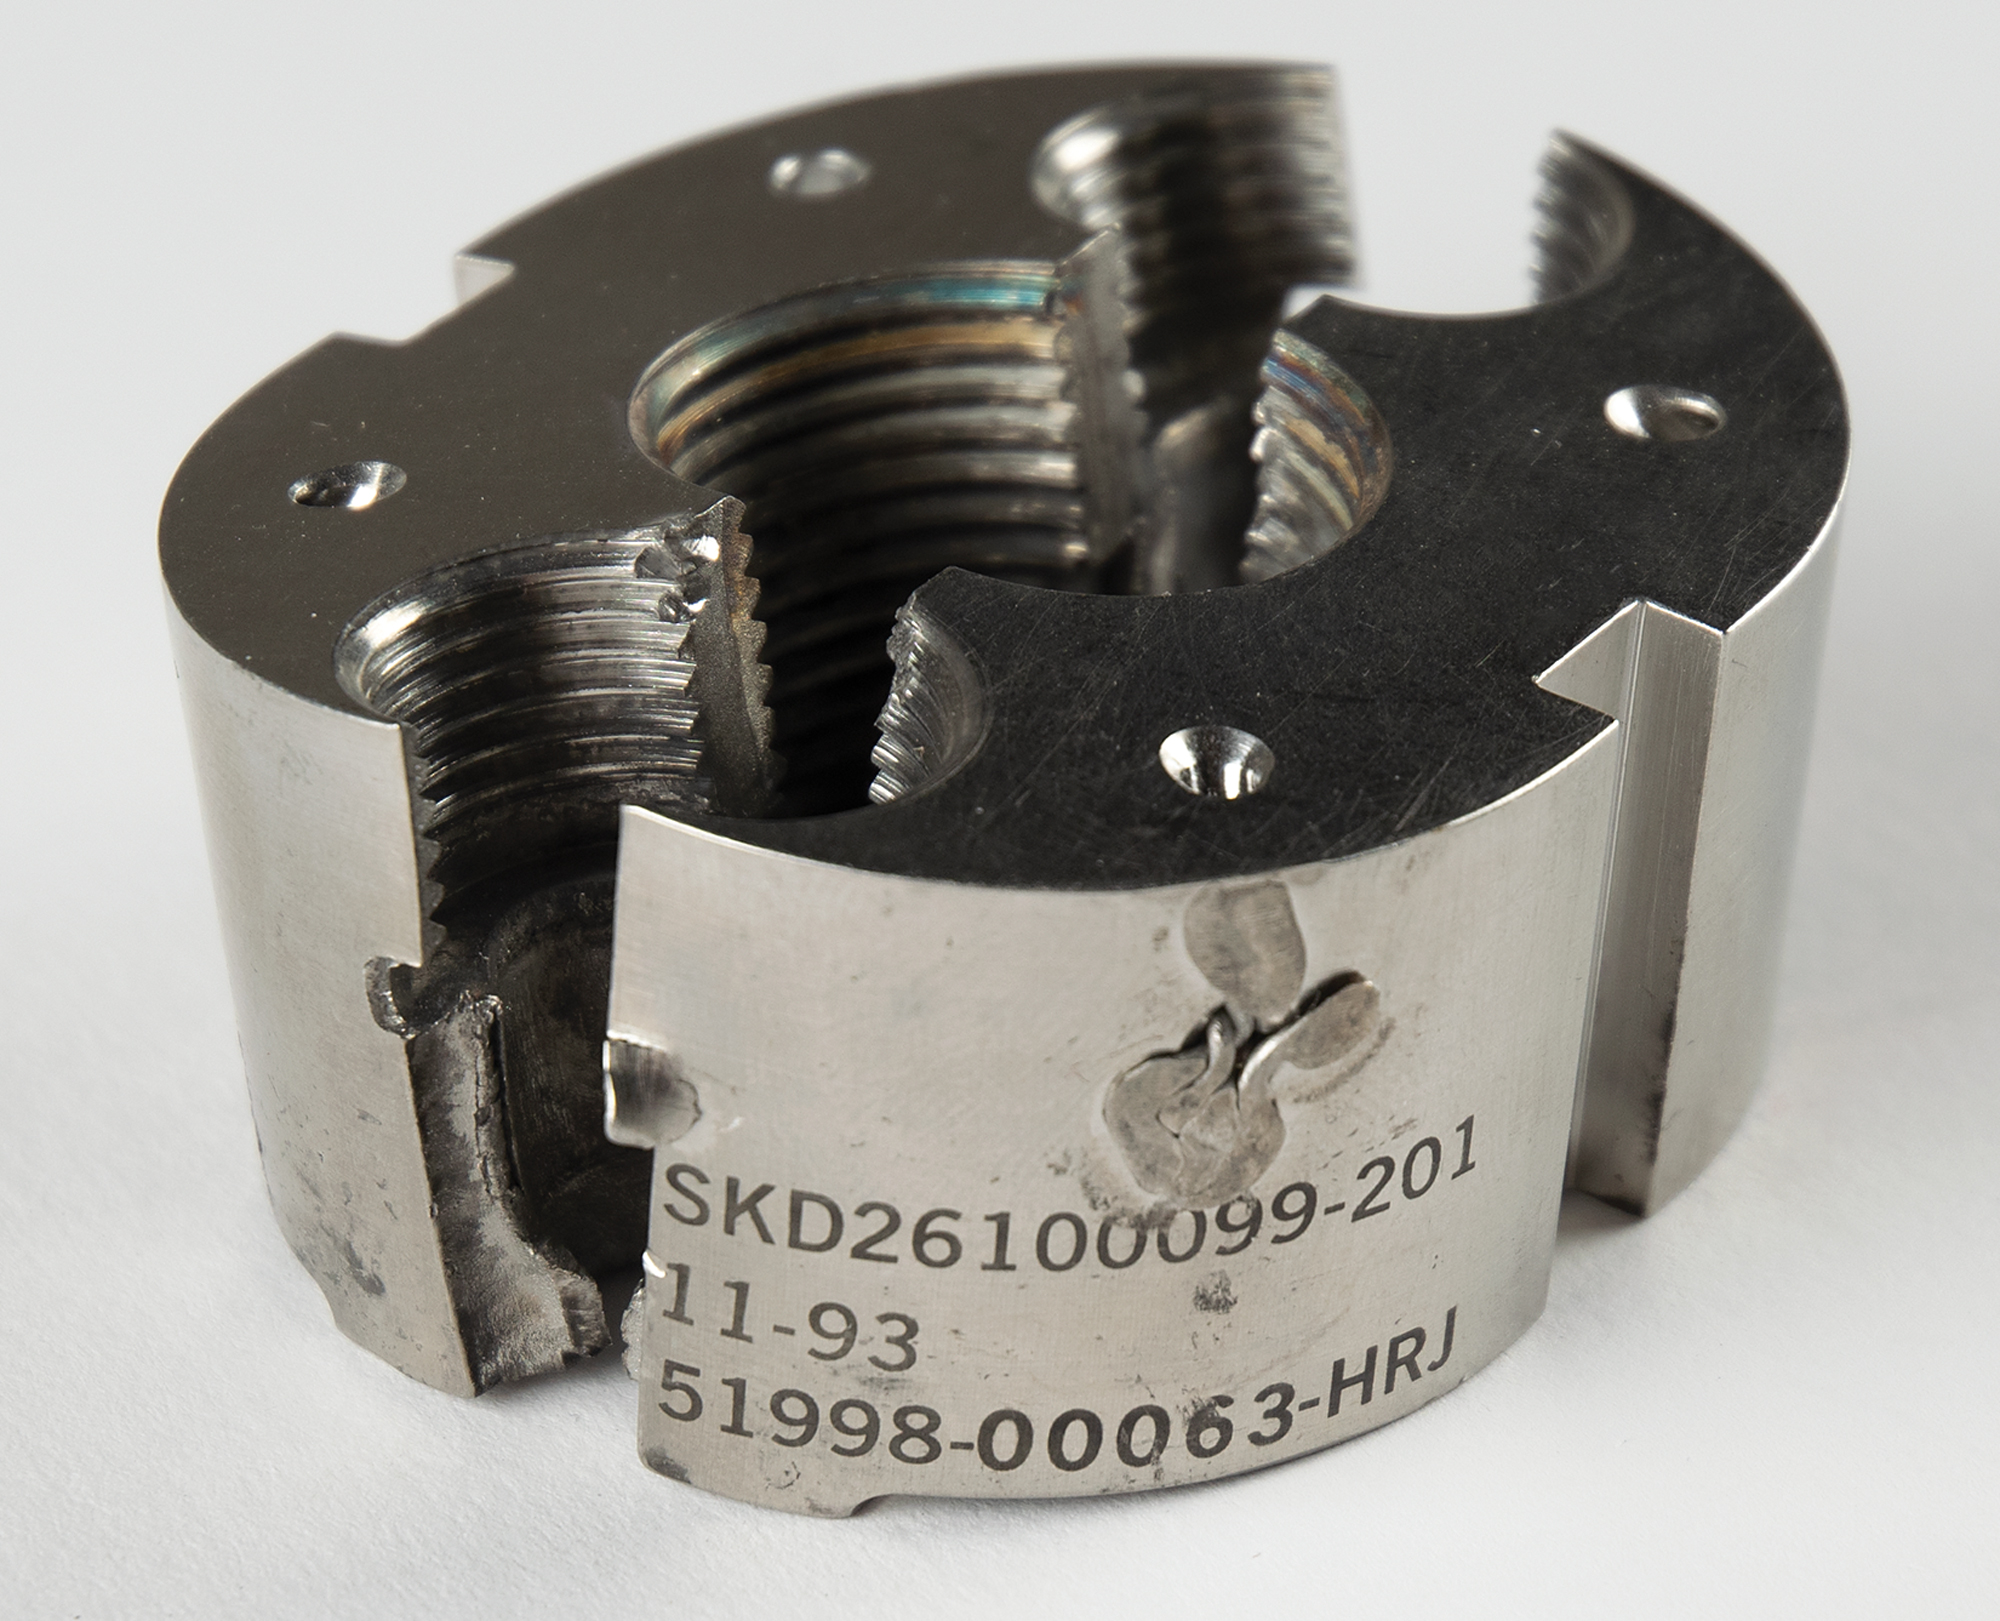
\includegraphics[width=0.4\textwidth]{figures/3454621_1.jpg}
    \caption{Boulon explosif ayant été utilisé sur les navettes spatiales américaines}
\end{figure}

\subsubsubsection{Non-pyrotechnique (mécanique / actionneurs)}

Les mécanismes non-pyrotechniques reposent sur des actionneurs, ressorts, latches ou systèmes cinématiques qui libèrent les
connections sans explosion. Ces solutions sont souvent utilisées dans des contextes où l’usage d’explosifs est indésirable ou
interdit.\\

\begin{itemize}
    \item \textbf{Mode d’activation :} Un système mécanique (servo-moteur, ressort à compression, actionneur linéaire) pousse ou
    désaccouple les éléments de fixation, libérant la contrainte.
    \item \textbf{Efforts mobilisés :} Forces généralement plus faibles et contrôlées, avec possibilité de modulation progressive
    des mouvements.
    \item \textbf{Avantages :} Moindre choc mécanique, possibilité de réversibilité ou de test au sol répétable.
    \item \textbf{Inconvénients :} Complexité mécanique accrue, risques d’enrayement ou d’erreur de synchronisation, besoins de
    commande et d’alimentation électrique supplémentaires.\\
\end{itemize}

Ce type de mécanisme est illustré par des solutions développées sur des projets étudiants ou petits lanceurs, où des serrures
mécaniques à bande associées à des actuateurs à fil résistif permettent un désaccouplement contrôlé avec faible impact
structurel \cite{EPFL_Separation}.

\subsubsection{Stratégies de séparation d’étages}

Au-delà du type de mécanisme utilisé pour rompre la liaison mécanique, la séquence de séparation joue un rôle majeur dans la
dynamique du vol. Deux stratégies opposées sont employées selon les architectures : la séparation à froid et à chaud
\cite{Multistage_Rocket}.

\subsubsubsection{Séparation à froid}

Dans une stratégie de séparation à froid, la séparation mécanique est effectuée avant l’allumage du moteur de l’étage supérieur.
L’étage inférieur termine sa combustion, se détache, puis le moteur du deuxième étage est mis en route après un court intervalle.

\begin{itemize}
    \item \textbf{Mode d'activations :} Séparation mécanique puis intervalle libre puis allumage du moteur supérieur.
    \item \textbf{Efforts mobilisés :} Efforts d’éloignement donnés par les dispositifs de séparation, puis poussée indépendante
    du moteur supérieur.
    \item \textbf{Avantages :} Isolation claire des phases de séparation et d’allumage, moins d’interactions thermiques ou
    mécaniques entre étages.
    \item \textbf{Inconvénients :} Nécessite un effort de séparation élevé pour assurer un éloignement suffisant avant l’allumage, ce qui
    peut imposer des dispositifs plus robustes et lourds.\\
\end{itemize}

Ce schéma est traditionnellement utilisé dans de nombreuses architectures occidentales (ex. Atlas, Titan, Saturn) où la finalité
est une séparation nette avant l’allumage moteur \cite{Multistage_Rocket}.

\subsubsubsection{Séparation à chaud}

Dans la séparation à chaud, le moteur de l’étage supérieur est allumé avant ou au moment de la séparation mécanique. Cette
approche utilise la poussée du moteur supérieur pour aider à éloigner les étages.\\

\begin{itemize}
    \item \textbf{Mode d'activations :} Allumage du moteur supérieur avant la séparation mécanique complète.
    \item \textbf{Efforts mobilisés :} Poussée continue transmise, ainsi qu’efforts de séparation mécanique.
    \item \textbf{Avantages :} Peut simplifier certaines interfaces mécaniques et augmenter l’impulsion disponible.
    \item \textbf{Inconvénients :} Interactions thermiques et dynamiques complexes entre jets moteurs et structure résiduelle ;
    demande une chonologie précise de la séquence de séparation.\\
\end{itemize}

Ce mode est caractéristique des architectures russes telles que Soyouz et Proton, et était prévu pour des programmes comme celui
de la fusée lunaire soviétque N1 \cite{Multistage_Rocket}. Elle est également la solution utiliser dans certains projets tel
que le lanceur Starship de SpaceX.

\begin{figure}[ht]
    \centering
    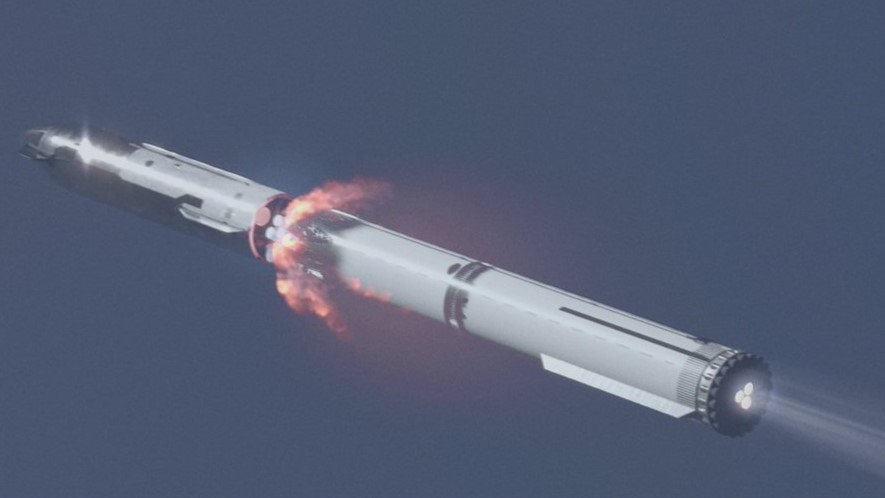
\includegraphics[width=0.9\textwidth]{figures/F3wgivuWkAAI7dq.jpg}
    \caption{Séparation à chaud du lanceur Starship de SpaceX}
\end{figure}

\subsubsection{Séparation à chaud sans connexion mécanique}

Parmi les diverses stratégies de séparation d'étage utilisées dans les lanceurs multi-étages, une approche particulière sans
connexion mécanique entre les étages a émergé dans certains contextes expérimentaux, notamment dans plusieurs projets américains
de petite échelle. Dans ce mode, les étages sont simplement empilés sans fixation structurelle rigide : l’étage supérieur repose
sur l’étage inférieur sans liaison mécanique formelle, et la séparation est obtenue uniquement par l’allumage du moteur du second
étage \cite{Whitman_2025_HotStagingModule}.L’absence de dispositifs de séparation classiques (boulons pyrotechniques, actionneurs,
ressorts) réduit drastiquement le nombre de sous-systèmes nécessaires pour réaliser la séparation, facilitant une simplification
mécanique attractive pour des équipes à ressources limitées.\\

L’effort mobilisé est essentiellement la poussée continue du moteur supérieur, qui doit non seulement accélérer le haut de la
fusée vers l’avant, mais aussi fournir l’impulsion relative nécessaire pour éloigner l’étage inférieur. Contrairement aux
mécanismes pyrotechniques ou mécaniques classiques, il n’y a pas de force transmise par une rupture contrôlée d’une liaison
structurelle : toute la dynamique de séparation dépend du flux de poussée du second étage.\\

Cette approche présente plusieurs avantages potentiels pour les lanceurs expérimentaux :
\begin{itemize}
    \item \textbf{Simplicité apparente du système de séparation :} l’élimination des éléments de séparation active (boulons,
    mécanismes, ressorts) réduit le nombre de pièces et donc les points de défaillance potentiels. Cela peut alléger la charge de
    conception et de fabrication dans un cadre associatif ou éducatif.
    \item \textbf{Réduction de la masse et de la complexité mécanique :} sans dispositifs de séparation dédiés, les interfaces
    entre étages restent minimalistes.
    \item \textbf{Facilité de test et d’intégration :} l’absence de mécanismes complexes permet des essais plus simples au sol,
    sans nécessiter de procédures de sécurité lourdes liées aux explosifs ou aux systèmes mécaniques sous tension.\\
\end{itemize}

Cependant, l’absence de liaison mécanique structurée entre les étages introduit des défis significatifs, qui sont particulièrement
critiques sur des véhicules à petite échelle :

\begin{itemize}
    \item \textbf{Absence de continuité structurelle :} sans fixation rigide, l’étage supérieur et l’étage inférieur ne partagent
    pas de lien structurel capable d’amortir ou de répartir les charges dynamiques. Cela implique que toute perturbation
    extérieure, vent latéral, irrégularité du vol ou micro-oscillation, peut provoquer une oscillation non atténuée du haut de
    l’étage avant séparation, ce qui peut affecter la trajectoire globale. À la différence des systèmes avec liaisons
    structurelles, où les étages restent couplés mécaniquement jusqu’à l’événement de séparation proprement dit, l’absence de
    cette contrainte rend le haut de la fusée plus sensible aux perturbations.
    \item \textbf{Contraintes sur la stabilité de trajectoire :} ce mode de staging exige une trajectoire dynamique parfaitement
    stabilisée avant l’allumage du moteur supérieur. La moindre erreur de centrage aerodynamique ou déséquilibre du véhicule peut
    se manifester sous forme de mouvement de tangage, lacet ou de roulis non atténués, car il n’existe pas de structure commune
    pour résorber ces effets.\\
\end{itemize}

Des travaux académiques récents illustrent l’intérêt de concevoir des modules de séparation chaude pour des fusées à deux étages
sans mécanismes de séparation traditionnels. Par exemple, une équipe universitaire a conçu un \textit{\og{}Hot Staging
Module\fg{}} en explorant des outils de simulation numérique (CFD) pour valider cette approche
\cite{Whitman_2025_HotStagingModule}. Ces projets soulignent l’intérêt de réduire le nombre de modes de défaillance liés aux
mécanismes classiques, mais insistent sur la nécessité d’une analyse dynamique approfondie du système de staging pour assurer la
stabilité et prédictibilité du comportement en vol.

\newpage

\subsubsection{Avantages et limitations des principaux modes et stratégies de séparation}

\begin{table}[h!]
\centering
\renewcommand{\arraystretch}{1.3}
\begin{tabular}{|p{2cm}|p{2.25cm}|p{2.25cm}|p{3.5cm}|p{3.5cm}|}
\hline
\textbf{Mode / \newline stratégie} &
\textbf{Mode d’activation} &
\textbf{Efforts mobilisés} &
\textbf{Avantages principaux} &
\textbf{Limitations principales} \\
\hline

Séparation pyrotechnique &
Détonation contrôlée &
Impulsion mécanique brusque &
Fiabilité élevée, séparation rapide, technologie éprouvée &
Chocs mécaniques importants, irréversibilité, contraintes réglementaires liées aux explosifs \\
\hline

Séparation mécanique &
Actionneur, ressort ou système cinématique &
Efforts progressifs et contrôlés &
Réduction des chocs, testabilité au sol, absence d’explosifs &
Complexité mécanique accrue, risques d’enrayement, besoins en énergie et en commande \\
\hline

Séparation à froid &
Séparation mécanique puis allumage moteur &
Efforts de séparation dédiés uniquement &
Découplage clair entre séparation et propulsion, interactions limitées &
Effort de séparation plus élevé requis, présence possible de systèmes auxiliaires (ullage) \\
\hline

Séparation à chaud &
Allumage moteur avant ou pendant la séparation &
Poussée moteur combinée à la séparation mécanique &
Réduction de l’effort de séparation, simplification partielle des sous-systèmes &
Contraintes thermiques et dynamiques, séquence de séparation critique \\
\hline

Séparation chaude sans connexion mécanique &
Allumage moteur du second étage uniquement &
Poussée moteur seule &
Simplicité structurelle maximale, masse réduite, peu de sous-systèmes &
Forte exigence de stabilité, sensibilité aux perturbations externes, domaine d’emploi restreint \\
\hline

\end{tabular}
\caption{Comparaison des principaux modes et stratégies de séparation d’étages}
\label{tab:separation_modes}
\end{table}

L’analyse comparative des principaux modes de séparation met en évidence l’absence de solution universelle, chaque approche
reposant sur un compromis entre simplicité mécanique, maîtrise dynamique et complexité opérationnelle.\\

Les systèmes pyrotechniques, largement éprouvés dans le domaine spatial industriel, offrent une séparation rapide et fiable, mais
au prix de chocs mécaniques élevés, d’une irréversibilité totale et de contraintes réglementaires incompatibles avec de nombreux
projets expérimentaux. À l’inverse, les solutions non-pyrotechniques réduisent les niveaux de choc et améliorent la testabilité,
mais introduisent une complexité mécanique et fonctionnelle qui peut devenir pénalisante dans des architectures légères et à
ressources limitées.\\

Du point de vue des stratégies de staging, la séparation à froid privilégie une séquence clairement découplée entre séparation et
propulsion, au prix d’efforts de séparation dédiés. La séparation à chaud, en exploitant directement la poussée du moteur
supérieur, permet de réduire ces efforts mais impose une gestion fine des interactions thermiques et dynamiques au moment de la
séparation.\\

Enfin, le hot staging sans connexion mécanique, observé dans certains projets expérimentaux, illustre une recherche de simplicité
extrême en supprimant tout dispositif de séparation dédié. Cette approche transfère toutefois l’essentiel des contraintes vers la
stabilité aérodynamique et inertielle du véhicule, rendant le système particulièrement sensible aux perturbations extérieures et
limitant fortement son domaine d’application.\\

Dans le contexte des lanceurs expérimentaux et des fusées sondes, ces constats soulignent que la problématique de la séparation
d’étages ne se résume pas à un choix technologique isolé, mais relève d’un équilibre global entre architecture, dynamique du vol
et contraintes opérationnelles. Cette analyse justifie l’exploration de solutions intermédiaires, capables de générer un effort
de séparation maîtrisé sans recourir à des dispositifs pyrotechniques ni à des mécanismes complexes, tout en limitant les
exigences imposées à la stabilité du véhicule.


\subsubsection{Principe de la solution étudiée : séparation assistée par aérofreinage}

L’état de l’art met en évidence une grande diversité de systèmes de séparation d’étages, reposant sur des compromis différents
entre fiabilité, complexité mécanique, maîtrise des efforts transmis et exigences sur la stabilité du véhicule. Aucune de ces
solutions ne s’impose comme universelle dans le cadre des lanceurs expérimentaux, où les contraintes de simplicité, de sûreté et
de moyens d’essai limités occupent une place centrale.\\

Dans ce contexte, le présent travail propose d’explorer une approche alternative, fondée sur l’exploitation des efforts
aérodynamiques disponibles en phase atmosphérique. Le principe de la séparation assistée par aérofreinage consiste à provoquer
une augmentation volontaire de la traînée sur l’étage inférieur, au moyen de dispositifs aérodynamiques déployables, afin de
créer une décélération différentielle entre les deux étages. Cette dissymétrie d’efforts aérodynamiques génère un effort
longitudinal relatif qui contribue à initier l’éloignement des étages de manière progressive, sans recours à des charges
pyrotechniques ni à des mécanismes énergétiques dédiés.\\

Afin de permettre l’évaluation expérimentale de ce principe dans des conditions représentatives d’un lanceur expérimental, le
projet SP-02 repose sur la réalisation d’une fusée bi-étage spécifiquement conçue comme vecteur d’essai. L’architecture retenue
intègre des aérofreins destinés à générer l’effort de séparation étudié, tout en conservant une continuité structurelle contrôlée
entre les étages jusqu’à l’événement de séparation. Un dispositif mécanique à ressort, indépendant du mécanisme aérodynamique et
activé de manière décalée, est également intégré afin de garantir la séparation effective du véhicule, y compris en cas
d’efficacité insuffisante du phénomène d’aérofreinage.\\

La compréhension et l’analyse de ce principe de séparation reposent directement sur les caractéristiques géométriques,
structurelles et aérodynamiques du vecteur expérimental. La section suivante est ainsi consacrée à la présentation du lanceur
SP-02, de sa philosophie de conception et de son rôle en tant que support d’expérimentation pour l’étude de la séparation
d’étages assistée par aérofreinage.

\newpage

\subsection{Présentation du lanceur SP02}
\label{sec:presentation_SP02}

\subsubsection{Cadre de lancement : le C’Space et ses contraintes}

Le développement du lanceur SP-02 s’inscrit dans le cadre de la campagne nationale \gls{C'Space}, organisée par
\gls{Planète Sciences} avec le soutien du \acrfull{CNES}. Cette campagne constitue aujourd’hui le principal, et pratiquement
l’unique, cadre de lancement accessible en France pour des projets de fusées expérimentales étudiantes. Elle fournit un
environnement réglementé permettant la réalisation d’essais en vol, sous réserve du respect d’un cahier des charges technique et
de sûreté particulièrement structurant.\\

La participation au \gls{C'Space} implique la conformité à un \acrfull{CDC} exigeant, couvrant notamment les aspects de sécurité
sol et vol, la robustesse des architectures retenues, la maîtrise des risques et la justification détaillée des choix techniques.
Les systèmes critiques du lanceur, en particulier ceux liés à la séparation d’étages, doivent ainsi faire l’objet d’analyses
documentées, d’essais préalables et d’une traçabilité complète. Certaines solutions, bien que pertinentes d’un point de vue
théorique ou industriel, peuvent se révéler difficilement compatibles avec ce cadre, notamment en raison des contraintes
réglementaires associées à l’utilisation de dispositifs pyrotechniques ou de mécanismes complexes.\\

Ce contexte impose également des contraintes fortes sur la philosophie de conception du lanceur. Le véhicule doit être
suffisamment simple et robuste pour garantir un niveau de sûreté acceptable, tout en restant instrumentable et exploitable du
point de vue expérimental. La reproductibilité des essais, la capacité à analyser les événements de vol et la récupération des
données constituent des critères déterminants dans l’évaluation des projets par les instances de suivi.\\

Ainsi, le cadre du \gls{C'Space} ne se limite pas à une opportunité de lancement, mais constitue un élément structurant de la
conception du lanceur SP-02. Les choix architecturaux retenus résultent directement de ce compromis entre exigences
réglementaires, contraintes opérationnelles et objectifs expérimentaux. La section suivante présente l’architecture générale du
lanceur SP-02, telle qu’elle a été définie pour répondre à ces contraintes tout en servant de support à l’étude de la séparation
d’étages assistée par aérofreinage.

\begin{figure}[h!]
    \centering
    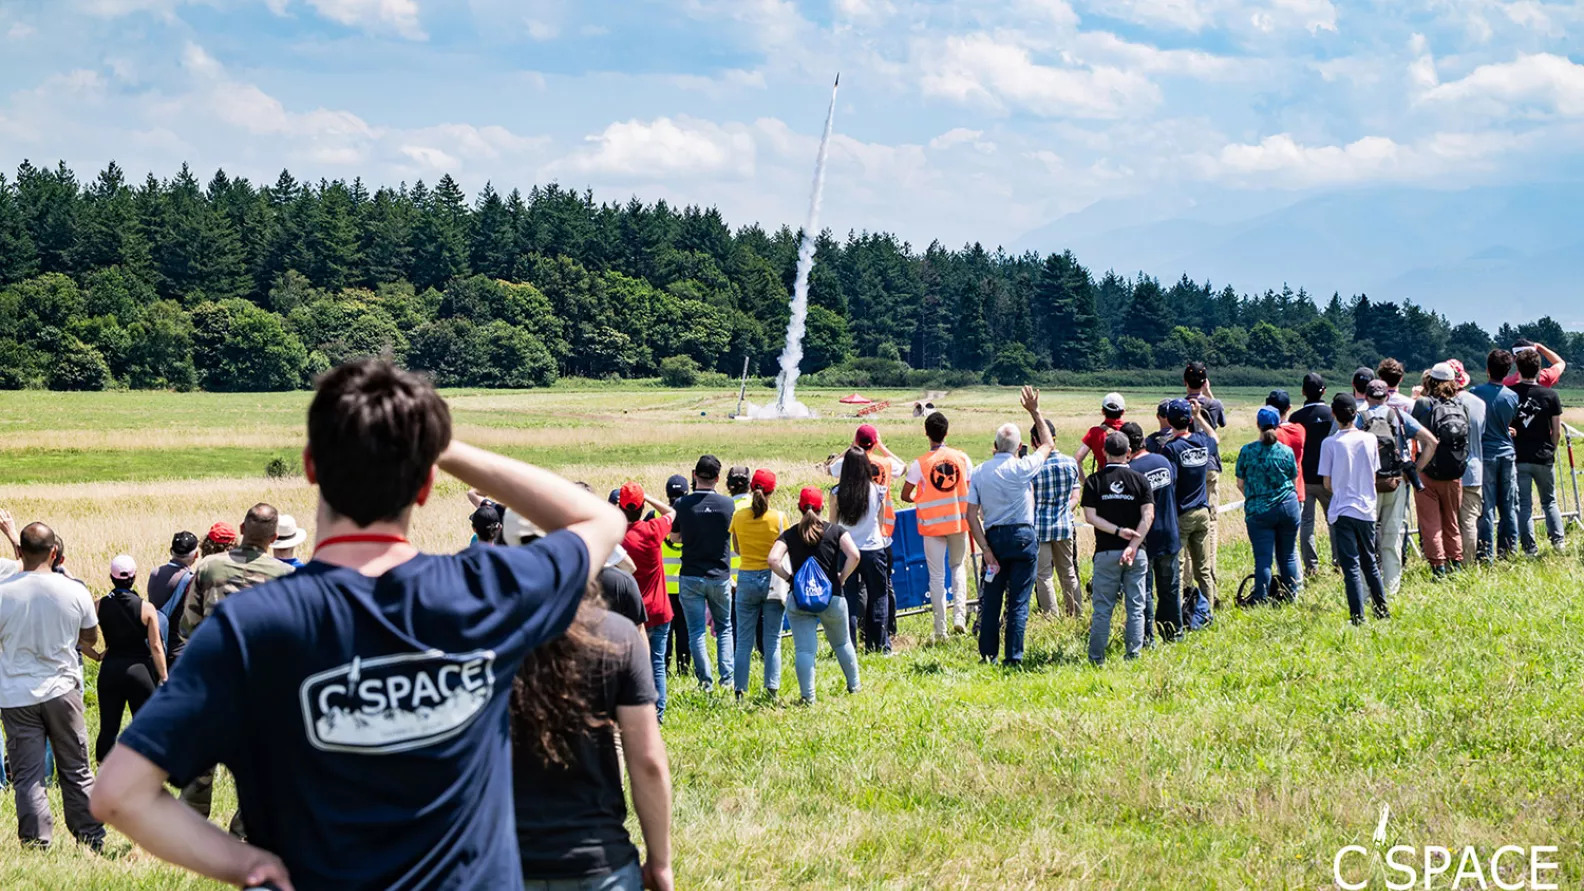
\includegraphics[width=0.7\textwidth]{figures/cspace-2024-1.jpg}
    \caption{Décollage d'une fusée expérimentale au C'Space 2024. \copyright CNES/C'Space/Thomas Labois}
\end{figure}

\subsubsection{Architecture générale du lanceur SP-02}

L’architecture repose sur une organisation claire en deux étages. Le premier étage assure la phase propulsive initiale et
constitue le support principal de l’expérience de séparation, en embarquant les dispositifs aérodynamiques étudiés. Le second
étage est un étage propulsif à part entière, permettant à la fois l’étude du comportement relatif lors de la séparation et la
poursuite du vol après celle-ci. Son intégration implique des fonctions spécifiques de commande et de sécurité liées à l’allumage
moteur, qui seront détaillées ultérieurement. Les architectures mécanique et électronique du lanceur SP-02 sont présentées dans les sections suivantes, dans la mesure
strictement nécessaire à la compréhension du principe étudié et des analyses menées par la suite.

\newpage

\subsubsubsection{Architecture mécanique}

Le premier étage du lanceur SP-02, d’une longueur totale de 1130 mm et d’un diamètre de 104 mm, est propulsé par un moteur
à ergole solide K570 - Pro54-5G, d'une poussée moyenne de 572 N, d'temps de combustion de 3.61~s et donc d'une impulsion totale de
2070 Ns, c'est un moteur de classe K. Le premier étage intègre également 4 surfaces aérodynamiques (ailerons) pour la stabilité en
vol, ainsi que 3 aérofreins déployables destinés à générer l’effort de séparation placé au dessus du moteur. Viens ensuite le bloc
de parachute assurant la récupération du premier étage, suivi du bloc électronique contenant l’ensemble des cartes de commande et
d’acquisition. Enfin, la partie haute du premier étage se caractérise par le système de séparation.

\begin{figure}[h!]
    \centering
    \begin{tikzpicture}
    
        \node at (0, 0) {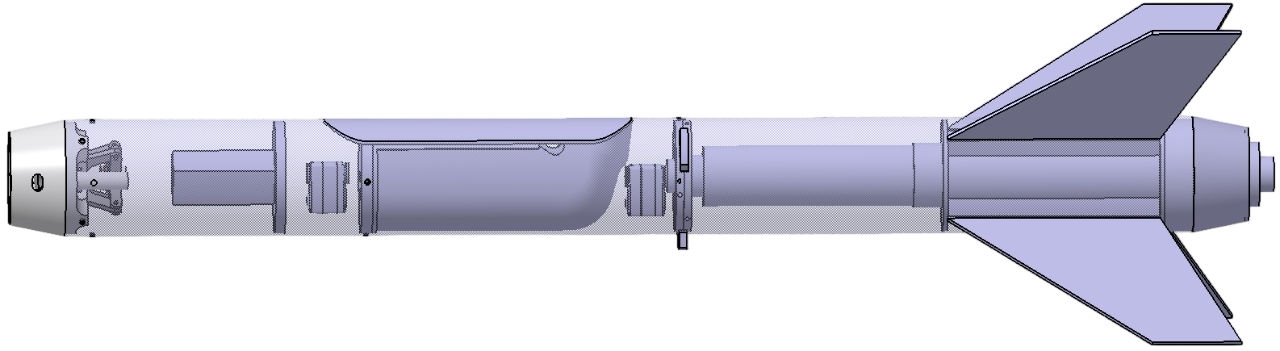
\includegraphics[width=\textwidth]{figures/catia_alpha.png}};
        
        \node (retreint_lbl)   at (+8.00, +2.5) {\textbf{Rétreint}};
        \node (bloc_propu_lbl) at (+4.30, +2.3) {\textbf{Bloc propulsion}};
        \node (propu_lbl)      at (+2.00, +1.5) {\textbf{Pro54-5G}};
        \node (aileron_lbl)    at (+2.00, -1.5) {\textbf{Ailerons (x4)}};
        \node (af_lbl)         at (+0.00, +2.3) {\textbf{Aérofreins (x3)}};
        \node (bloc_para_lbl)  at (-2.00, +1.5) {\textbf{Bloc parachute}};
        \node (bloc_elec_lbl)  at (-6.00, +2.3) {\textbf{Bloc électronique}};
        \node (bloc_sepa_lbl)  at (-6.00, -1.5) {\textbf{Bloc séparation}};

        \node (bloc_propu_box) at (+5.10, 0.00) [minimum width=35mm, minimum height=18mm, rectangle, line width=2, draw=red] {};
        
        \draw[red, ->, line width=1.5] (retreint_lbl.south)   -- (+7.20, +0.60);
        \draw[red, ->, line width=1.5] (bloc_propu_lbl.south) -- (bloc_propu_box.140);
        \draw[red, ->, line width=1.5] (propu_lbl.south)      -- (+2.20, +0.00);
        \draw[red, ->, line width=1.5] (aileron_lbl.east)     -- (+6.50, -1.50);
        \draw[red, ->, line width=1.5] (af_lbl.south)         -- (+0.30, +0.60);
        \draw[red, ->, line width=1.5] (bloc_para_lbl.south)  -- (-2.00, +0.00);
        \draw[red, ->, line width=1.5] (bloc_elec_lbl.south)  -- (-5.30, +0.00);
        \draw[red, ->, line width=1.5] (bloc_sepa_lbl.north)  -- (-7.30, +0.00);

    \end{tikzpicture}
    \caption{Vue du premier étage sur \acrshort{CATIA}}
    \label{fig:sp02_s1_ork}
\end{figure}

Le second étage, d’une longueur totale de 992 mm et d’un diamètre de 84 mm, est propulsé par un moteur 144G150 - Pro24-6G de la
même gamme que le moteur du premier étage. Il développe une poussée moyenne de 147~N pour un temps de combustion de 0.969~s, soit
une poussée totale de 144~Ns, c'est un moteur de classe G. Le second étage intègre une coiffe conique en tête faite en fibre de
verre et une pointe en aluminium, ainsi que 4 ailerons pour la stabilité en vol. Le bloc parachute assure la récupération de
l’étage, tandis que le bloc électronique contient les mêmes cartes que le premier étage afin de faciliter le développement. La
partie basse du second étage est quant à elle dédiée à l’interface de séparation avec le premier étage.

\begin{figure}[h]
    \centering
    \begin{tikzpicture}
    
        \node at (0, 0) {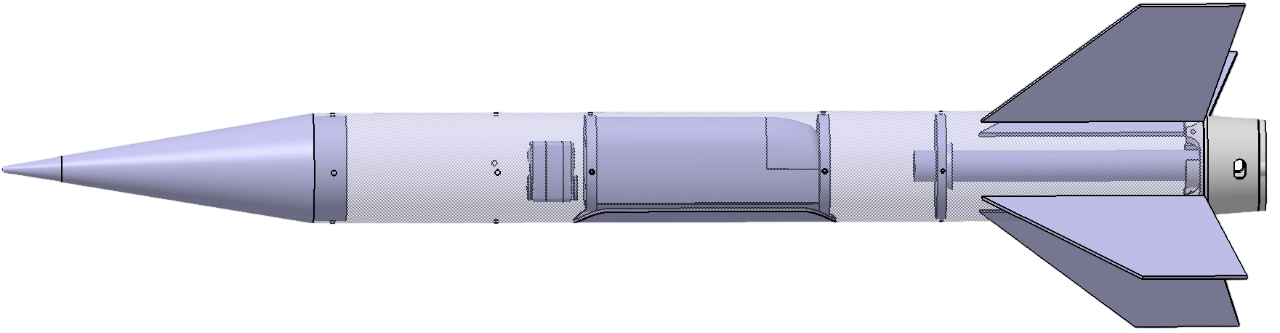
\includegraphics[width=\textwidth]{figures/catia_beta.png}};
        
        \node (bloc_sepa_lbl)   at (+8.00, +2.5) {\textbf{Interface de séparation}};
        \node (propu_lbl)       at (+4.30, +2.3) {\textbf{Pro24-6G}};
        \node (bague_propu_lbl) at (+3.00, +1.5) {\textbf{bague de centrage}};
        \node (aileron_lbl)     at (+2.00, -1.5) {\textbf{Ailerons (x4)}};
        \node (bloc_para_lbl)   at (+1.00, +2.3) {\textbf{Bloc parachute}};
        \node (bloc_elec_lbl)   at (-2.00, +1.5) {\textbf{Bloc électronique}};
        \node (coiffe_lbl)      at (-5.00, +2.3) {\textbf{Coiffe conique}};
        \node (pointe_alu_lbl)  at (-6.00, -1.5) {\textbf{Pointe aluminium}};

        \draw[red, ->, line width=1.5] (bloc_sepa_lbl.south)    -- (+7.40, +0.60);
        \draw[red, ->, line width=1.5] (propu_lbl.south)        -- (+5.20, +0.00);
        \draw[red, ->, line width=1.5] (bague_propu_lbl.south)  -- (+3.70, +0.00);
        \draw[red, ->, line width=1.5] (aileron_lbl.east)       -- (+6.50, -1.00);
        \draw[red, ->, line width=1.5] (bloc_para_lbl.south)    -- (+0.30, +0.60);
        \draw[red, ->, line width=1.5] (bloc_elec_lbl.south)    -- (-2.50, +0.00);
        \draw[red, ->, line width=1.5] (coiffe_lbl.south)       -- (-5.30, +0.00);
        \draw[red, ->, line width=1.5] (pointe_alu_lbl.north)   -- (-7.30, +0.00);

    \end{tikzpicture}
    \caption{Vue du second étage sur \acrshort{CATIA}}
    \label{fig:sp02_s2_ork}
\end{figure}

L'ensemble du lanceur SP-02 présente une longueur totale de 2062 mm et une masse théorique au décollage d'environs 9.3 kg, dont
6.9 kg pour le premier étage et 2.4 kg pour le second étage. 

\newpage

\subsubsubsection{Architecture électronique et instrumentation}

[ A FAIRE ]

\newpage

\subsubsection{Phase de vol}

Le vol de la fusée SP-02 se déroule selon six phases successives représentées dans la figure suivante. Ce découpage permet
d’identifier clairement les séquences critiques du lanceur et de situer la phase de séparation d’étages dans le contexte global
du vol.

\begin{figure}[h!]
    \centering
    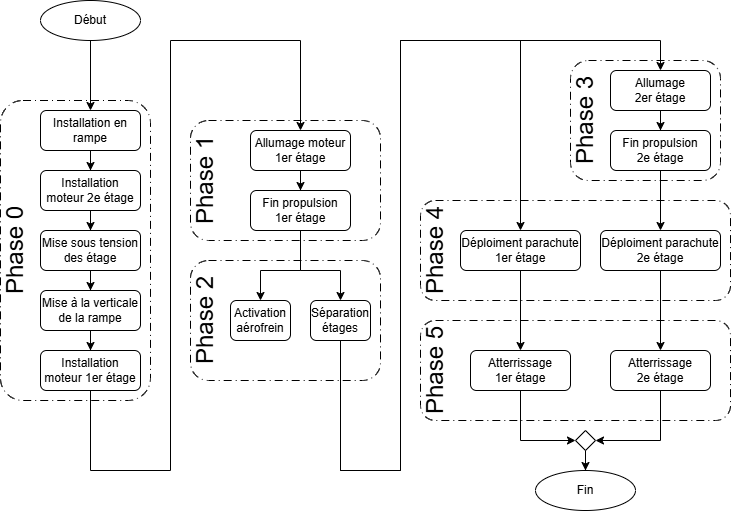
\includegraphics[width=\textwidth]{figures/Phase_vol.drawio.png}
    \caption{Phases de vol du lanceur SP-02}
    \label{fig:phases_vol_sp02}
\end{figure}

On distingue ainsi les phases suivantes :
\begin{itemize}
    \item \textbf{Phase 0 :} Préparation et mise en condition du système.
    \item \textbf{Phase 1 :} Propulsion et ascension du premier étage.
    \item \textbf{Phase 2 :} Séparation des étages.
    \item \textbf{Phase 3 :} Allumage et propulsion du second étage.
    \item \textbf{Phase 4 :} Ouverture des parachutes et descente des étages.
    \item \textbf{Phase 5 :} Atterrissage et récupération des étages.
\end{itemize}

\subsection{Attendus du projet, livrables et structuration du PMI}

Cette section a pour objectif de clarifier explicitement les attendus du Projet Master Innovation, les livrables associés, ainsi
que la manière dont le document est structuré afin de répondre de façon cohérente et progressive au sujet proposé. Elle
constitue un point de verrouillage méthodologique du rapport, en définissant précisément les objectifs poursuivis et le
périmètre de l’étude.

\subsubsection{Objectifs et périmètre de l’étude}

Le présent \acrshort{PMI} vise à évaluer la faisabilité technique et la pertinence expérimentale d’un système de séparation
d’étages de fusée reposant sur le principe de l’aérofreinage, dans le contexte d’un lanceur expérimental. L’objectif n’est pas
de proposer une solution industrialisable, mais de déterminer si une telle expérience peut être mise en œuvre dans des conditions
réalistes et conduire à l’obtention de données exploitables.\\

Dans ce cadre, le travail mené s’articule autour de plusieurs livrables principaux :
\begin{itemize}
    \item la conception et la réalisation de \textbf{prototypes fonctionnels} des systèmes de séparation et d’aérofreinage,
    intégrant leurs dispositifs de commande électroniques ainsi que la chaîne de mesure associée ;
    \item la production de \textbf{résultats de simulations numériques} permettant de caractériser les efforts
    aérodynamiques générés par les aérofreins et leur influence sur le comportement du lanceur ;
    \item la réalisation d’\textbf{analyses structurelles} visant à vérifier la tenue mécanique des éléments critiques et la
    cohérence globale de l’architecture retenue ;
    \item une \textbf{analyse globale des performances attendues}, des limites identifiées et de la pertinence du principe de
    séparation par aérofreinage dans un cadre expérimental.\\
\end{itemize}

\subsubsection{Structuration du travail et du document}

Le projet SP-02 mobilise des compétences variées en mécanique, aérodynamique, électronique et instrumentation, ce qui a conduit
à une organisation du travail fondée sur la spécialisation des membres selon ces domaines. La structure du document ne reflète
toutefois pas directement cette répartition interne, mais vise à proposer une lecture progressive et cohérente du projet. Les
différentes contributions y sont ainsi articulées autour d’un raisonnement global, depuis la conception des systèmes jusqu’à
l’analyse des résultats et aux réalisations.\\

La partie 2 est consacrée à la conception des systèmes de séparation et d’aérofreinage, ainsi qu’aux fonctions de séquencement
et de commande associées. Elle vise à présenter les choix architecturaux retenus et à définir les systèmes étudiés, tant du
point de vue mécanique qu’électronique.\\

La partie 3 présente la méthodologie employée pour étudier le fonctionnement des systèmes conçus. Elle regroupe les hypothèses
de modélisation, les approches numériques retenues pour les études aérodynamiques et structurelles, ainsi que les éléments
relatifs au processus expérimental envisagé. Cette partie a pour objectif de préciser le cadre d’analyse dans lequel les
résultats sont obtenus.\\

La partie 3 est consacrée à la méthodologie d’étude et de validation des systèmes conçus. Elle regroupe, au sein d’un même
ensemble cohérent, les hypothèses de modélisation retenues pour les études aérodynamiques et structurelles, ainsi que la
définition de la chaîne de mesure expérimentale envisagée pour la validation physique de l’expérience. Cette partie vise à
expliciter le cadre dans lequel les analyses numériques sont menées et à montrer comment elles s’articulent avec les moyens de
mesure prévus afin d’aboutir à des données exploitables.\\

Enfin, la partie 5 regroupe l’ensemble des réalisations concrètes issues du projet, incluant la fabrication des systèmes
mécaniques, le développement des systèmes électroniques et logiciels, ainsi que leur intégration. Cette partie permet de relier
les études menées aux éléments effectivement produits et d’apprécier la cohérence entre conception, analyses et mise en œuvre.\\

L’enjeu du PMI ne réside pas uniquement dans la réalisation d’études prises isolément, mais dans la capacité à mettre en regard
les différents résultats obtenus. Les choix de conception, les hypothèses aérodynamiques et les analyses structurelles sont
ainsi articulés afin d’éclairer progressivement le comportement du système étudié. La structuration du document vise à
accompagner cette démarche, en proposant une lecture cohérente permettant d’apprécier la faisabilité de l’expérience de
séparation par aérofreinage et la qualité des données susceptibles d’en être issues.

\newpage
